% Explainability and Interpretability
% Author: Adnan Ghribi

\label{sec:explainability}

Explainability is critical for deploying machine learning in safety-critical accelerator environments. This section presents an explainability framework combining global feature importance (SHAP), local instance explanations (LIME), and physics-grounded interpretation.

\subsection{Feature Importance Analysis with SHAP}

SHapley Additive exPlanations (SHAP) assigns feature importance values based on Shapley values from cooperative game theory, providing theoretically consistent explanations for model predictions~\cite{shap}.

\subsubsection{Global Feature Importance}

We compute SHAP values for all \MetricZeroSixBinaryClassificationNFeatures{} features across the test set, for a per-fault-category Random Forest classifier trained with a leakage-safe split, to identify globally important predictors. Figure~\ref{fig:shap_summary} shows the top features ranked by mean absolute SHAP value.

\begin{figure}[t]
    \centering
    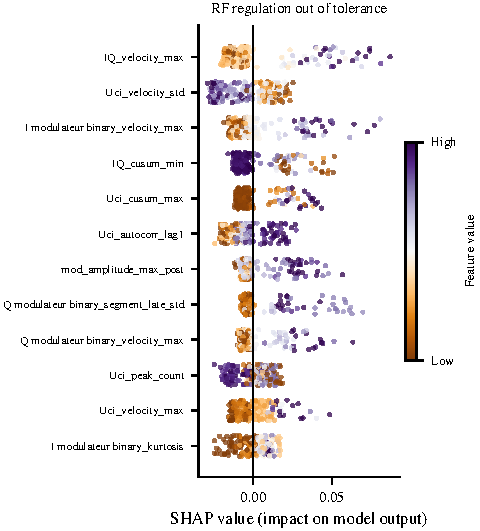
\includegraphics[width=\linewidth]{figures/shap_summary.pdf}
    \caption{SHAP summary (beeswarm) plot for \textit{RF regulation out of tolerance} (the largest category, n=591), from the same one-vs-rest, leakage-safe-split Random Forest used for the physics-group breakdown (Table~\ref{tab:physics_group_shap}, Sec.~\ref{sec:results}). Color indicates feature value (purple=high, orange=low); the x-axis shows each point's impact on model output. Shown for one representative, well-populated category rather than all seven to keep the figure legible; the full 7-category physics-group breakdown is tabulated separately.} % MANUAL: "591"/"7" are real, already macro-cited counts elsewhere (Sec. 1/6), repeated here as plain prose inside a caption
    \label{fig:shap_summary}
\end{figure}

Key findings, grouped by the actual \texttt{engineer\_features()} code section that produced each feature (Effective Decay, Detuning, Microphonics, RF Mismatch, Modulator Command, Phase Stability, RF Power Flow, Statistical, Temporal, Metadata/Status -- Sec.~\ref{sec:methodology}) rather than a substring-name heuristic, and reported as per-feature-mean importance rather than the group sum:

\begin{itemize}
    \item \textbf{Why per-feature-mean, not group sum}: the seven named physics-informed families total only \MetricOneZeroPhysicsGroupShapNFeaturesPhysicsInformedTotal{} features combined, versus \MetricOneZeroPhysicsGroupShapNFeaturesStatistical{} Statistical and \MetricOneZeroPhysicsGroupShapNFeaturesTemporal{} Temporal features -- roughly a 20:1 imbalance (full per-group breakdown in Sec.~\ref{sec:methodology}). % MANUAL: 20:1 is a rounded summary of the macro-cited counts, not a separate manifest metric
Summing SHAP importance by group structurally favors Statistical/Temporal regardless of how informative any individual physics-informed feature is; dividing by group size (per-feature mean) is the fairer basis for a "which group matters most" claim, and changes the answer substantially (Table~\ref{tab:physics_group_shap}).
    \item \textbf{A physics-informed family is dominant for four of seven fault categories} on a per-feature-mean basis: RF Mismatch for fast external cutoff (\MetricOneZeroPhysicsGroupShapFastExternalCutoffTopGroupMeanPct\%); Modulator Command for RF authorization absent (\MetricOneZeroPhysicsGroupShapRfAuthorizationAbsentTopGroupMeanPct\%); and Effective Decay for both cavity quench/breakdown (\MetricOneZeroPhysicsGroupShapCavityQuenchBreakdownTopGroupMeanPct\%, physically consistent with a quench's defining rapid-collapse signature) and RF regulation out of tolerance (\MetricOneZeroPhysicsGroupShapRfRegulationOutOfToleranceTopGroupMeanPct\%) -- these two categories converging on the same physics-informed family is itself notable, since nothing in the taxonomy assumes they should. The remaining three categories are genuinely Statistical-dominated: pickup threshold (\MetricOneZeroPhysicsGroupShapPickupThresholdTopGroupMeanPct\%), vacuum threshold (\MetricOneZeroPhysicsGroupShapVacuumThresholdTopGroupMeanPct\%) -- neither has a dedicated physics-informed feature family in this pipeline (Appendix~\ref{appendix:features}), so any physical signal from those two categories can only appear in the generic Statistical group -- and RF safety threshold exceeded (\MetricOneZeroPhysicsGroupShapRfSafetyThresholdExceededTopGroupMeanPct\%), which does have a matching family (RF Power Flow) but Statistical edges it out regardless.
    \item \textbf{The literal top-ranked individual features per category are a separate question from group dominance}, and are still often drawn from the large Temporal/Statistical groups even where a physics-informed family wins on a per-feature-mean basis -- e.g. cavity quench/breakdown's single highest-SHAP individual features are \texttt{Ucav\_accel\_max} and \texttt{Q\_Ucav\_binary\_accel\_max} (both Temporal) and \texttt{Ucav\_autocorr\_lag1} (Statistical), even though Effective Decay is the top group on average. Per-feature-mean answers "which family is most reliably informative, member for member"; the individual ranking answers "which single feature ranks highest" -- these are both legitimate, different questions, and we report both rather than only the more flattering one.
\end{itemize}

This is a data-driven finding, not an assumed one, and a substantially different one than an unnormalized group-sum comparison would suggest (Sec.~\ref{sec:methodology}). None of these physics-informed families include a loaded quality factor ($Q_L$), which -- as noted in Sec.~\ref{sec:methodology} -- is not physically well-defined for the postmortem fault transients this pipeline analyzes and is not among the implemented features.

\subsubsection{Per-Fault-Type Feature Importance}

SHAP analysis stratified by fault type (Table~\ref{tab:physics_group_shap}, Sec.~\ref{sec:results}) shows the dominant feature group differs by category and is generally consistent with each category's distinct physical signature: both cavity quench/breakdown and RF regulation out of tolerance are Effective-Decay-dominated (an abrupt voltage collapse and a control-loop deviation are both, at the feature level, rapid-change-of-Ucav events); RF authorization absent is Modulator-Command-dominated, tying it directly to the RF drive demand rather than the cavity's measured response; fast external cutoff is RF-Mismatch-dominated, consistent with an external interlock event registering as a reflected/forward-power imbalance; and vacuum/pickup-threshold categories -- lacking a dedicated physics feature family for the signals that literally define them -- fall back to generic statistical structure, as does RF safety threshold exceeded despite having a matching (but not dominant) physics-informed family.

\subsection{LIME for Local Explanations}

Local Interpretable Model-Agnostic Explanations (LIME)~\cite{lime} generates instance-level explanations by fitting a local linear model around one individual prediction. Fig.~\ref{fig:lime_example} shows one representative example -- a confidently-classified true positive -- rather than a systematic sweep over every misclassified event, which is future work (Sec.~\ref{sec:conclusion}).

\begin{figure}[t]
    \centering
    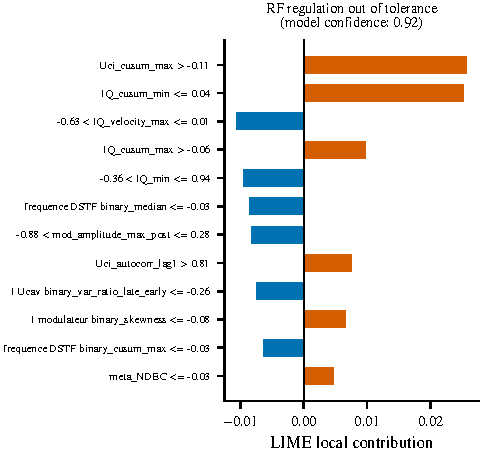
\includegraphics[width=\linewidth]{figures/lime_example.pdf}
    \caption{LIME local explanation for one confidently-classified \textit{RF regulation out of tolerance} test event (same model as Fig.~\ref{fig:shap_summary}), showing the discretized feature-threshold rules with the largest local contribution. Orange bars support the prediction, blue bars oppose it.}
    \label{fig:lime_example}
\end{figure}

Analysis of the root-cause classifier's confusion pairs (Sec.~\ref{sec:results}) shows the dominant confusion is between the two largest categories: \textit{RF regulation out of tolerance} events are misclassified as \textit{RF authorization absent} in 8 of 313 % MANUAL: confusion counts from a single held-out split (analysis/results_manifest/10_phase3_weakness_diagnosis.yaml meta.confusion.root_cause), not currently exposed as manifest metrics
test events -- a real physical overlap between the two largest categories, not a random minority-class artifact -- while each of the four rarest categories has 2-3 events routed into the majority class, consistent with ordinary class-imbalance bias. % MANUAL: same source as above (10_phase3_weakness_diagnosis.yaml confusion counts), not yet a manifest metric
A systematic LIME sweep specifically over these confusion pairs, to test whether they share overlapping statistical-feature contributions, is running against the corrected V7 pipeline as of this writing (Phase A/B/C LIME extraction, launched 2026-09-10) and its results will be added once complete; not yet asserted here.

\subsection{Saliency for Deep Architectures}

Gradient-based saliency ($\partial\text{output}/\partial\text{input}$, per fault-category output head) is computed for all four phaseD deep architectures (CNN, CNN-LSTM, MLP, Transformer) over 200 sampled test events each, classified through the same physics-group taxonomy used for the classical-model SHAP breakdown above (Sec.~\ref{sec:methodology}), for a direct cross-method comparison. Group-sum saliency is Temporal-dominated for all four architectures (59.9\%--63.1\% of total saliency magnitude: CNN 60.6\%, CNN-LSTM 63.1\%, MLP 61.1\%, Transformer 59.9\%) % MANUAL: percentages read directly off the saliency .npz archives (step_10_phaseD/*/saliency_*.npz), computed with the SHAP script's own get_physics_group() classifier; not yet exposed as a results-manifest metric, unlike every macro-cited number elsewhere in this section
-- the same structural pattern SHAP shows for every classical-model category, and expected for the same reason (Temporal alone is \MetricOneZeroPhysicsGroupShapNFeaturesTemporal{} of \MetricZeroSixBinaryClassificationNFeatures{} features). This cross-method agreement between two structurally different attribution approaches (perturbation-based SHAP on tree ensembles, gradient-based saliency on neural networks) is a modest but real corroboration that the group-size imbalance, not model-specific behavior, drives the sum-based ranking. One architecture-specific finding worth flagging rather than smoothing over: the MLP's single highest-saliency feature is \texttt{meta\_KPI}, an acquisition-quality metadata field (Sec.~\ref{sec:system_description}), not a physics measurement -- the other three architectures' top feature is a genuine Temporal or Statistical physical measurement. This does not necessarily indicate a problem (KPI may correlate with real fault precursors indirectly), but is a concrete point to check before treating the MLP variant's explanations as equally physically grounded as the other three.

\subsection{Physics-Grounded Interpretation}

To ensure that model decisions align with physical plausibility, we validate feature importance against known LLRF physics at the signal-group level rather than asserting specific classical quantities that are not implemented in this pipeline:

\begin{itemize}
    \item \textbf{Effective-decay features} (Sec.~\ref{sec:methodology}) are the top per-feature-mean group for cavity quench/breakdown, physically consistent with a quench's defining rapid voltage-collapse signature, even though the single highest-ranked individual features there are drawn from the (much larger) Temporal group of generic derivative statistics (acceleration, velocity of cavity voltage) -- both point to the same underlying physical mechanism, a rapid change in cavity voltage, described at different levels of feature engineering.
    \item \textbf{Modulator-command features dominating RF authorization absent} is consistent with the category's name: it is defined by the RF regulation loop's own authorization state, so features describing the drive demand itself (rather than the cavity's measured response) are a physically direct signal. \textbf{RF regulation out of tolerance}, despite a similar name, is Effective-Decay-dominated rather than Modulator-Command-dominated -- the deviation itself is better captured by how the cavity voltage is changing than by the drive command that provoked it.
    \item \textbf{Statistical features dominate three categories} -- vacuum threshold, pickup threshold, and RF safety threshold exceeded -- none of which has a \emph{dominant} dedicated physics-informed feature family in this pipeline (RF safety threshold exceeded has a matching, but not winning, RF Power Flow family; the other two have none at all) -- a taxonomy gap for two of the three, not necessarily evidence that these faults manifest as a diffuse statistical change rather than through a specific physical mechanism.
    \item We explicitly do not compute or cite a loaded quality factor ($Q_L$) as an implemented feature: as discussed in Sec.~\ref{sec:methodology}, the standard exponential-decay-based $Q_L$ calculation requires a free cavity decay with the drive/loop disengaged, which does not describe the postmortem fault transients this pipeline analyzes (the loop remains closed and active throughout). $Q_L$ remains measurable on SPIRAL2's CW cavities by other standard means -- a frequency-domain bandwidth sweep, or a deliberately loop-opened decay test -- but those require dedicated measurements outside this pipeline's postmortem-only data, so no such feature exists in the pipeline's feature set.
\end{itemize}

\subsection{Explainability for Operator Trust}

The explainability framework serves several practical purposes:

\begin{enumerate}
    \item \textbf{Model Validation}: Physics-grounded validation ensures that ML models align with domain knowledge, preventing deployment of models that achieve accuracy through non-physical shortcuts.

    \item \textbf{Operator Trust}: Real-time explanations (SHAP values, feature importance) accompany predictions, allowing operators to verify that decisions are based on expected physical indicators.

    \item \textbf{Failure Diagnosis}: LIME explanations for misclassifications reveal model weaknesses, guiding targeted improvements (e.g., collecting more examples of rare fault types).

    \item \textbf{Knowledge Discovery}: Feature importance analysis can surface candidate fault mechanisms worth further physics review, informing hardware improvements and operational procedures.
\end{enumerate}

This explainability approach distinguishes our work from black-box ML applications in accelerator physics and demonstrates that high accuracy and interpretability are not mutually exclusive.
